%% Q1
Evaluation collects evidence about learning in order to make judgements and \textbf{take decisions}: about promotion, selection, remedial teaching, improvement of methods and curriculum, and so on. Evaluation is essentially a \emph{decision-making} process.

%% Q2
\textbf{Readiness} of the learner is the foremost condition of learning. It covers physical, mental, emotional and motivational preparedness (Thorndike's \emph{Law of Readiness}). Without it, even the best teaching does not produce learning.

%% Q3
A student's questions show curiosity and active thinking. A good teacher \textbf{encourages continued questioning}, which sustains inquiry and critical thinking, and answers patiently rather than suppressing or diverting the student.

%% Q4
In the \textbf{heuristic method} (H.~E.~Armstrong; Greek \emph{heurisko}, ``I discover'') the students themselves \textbf{strive to find out the solution}, behaving like discoverers. The teacher only guides.

%% Q5
Learning is defined as a relatively permanent \textbf{modification of behaviour} resulting from experience. Effective learning brings desirable change in the learner's knowledge, skills and attitudes, not merely recall or examination scores.

%% Q6
Deduction moves from \textbf{general to specific}: a rule or principle is stated first and then applied to particular examples. Induction moves from specific to general.

%% Q7
\textbf{Fundamental (basic or pure) research} aims at extending knowledge and \textbf{building or testing theory}, without regard to immediate practical application.
\why{Action research solves immediate local problems; applied research solves practical problems; historical research studies the past.}

%% Q8
A \textbf{bibliography} lists all the sources consulted for the research, \emph{whether or not} they are cited in the text. \emph{References} include only the works actually cited.

%% Q9
Every option except (C) describes an ethical practice. \textbf{Avoiding reliable information}, i.e.\ deliberately ignoring or suppressing trustworthy data, is unethical because it biases the findings.

%% Q10
\textbf{Snowball sampling} is a \textbf{non-probability} technique: each participant refers further participants from their own network. It is used for hidden or hard-to-reach populations.

%% Q11
To study the actual classroom teaching--learning \emph{process}, the researcher must observe it directly as it happens, using an \textbf{observation schedule} (e.g.\ Flanders' Interaction Analysis Categories).

%% Q12
The \textbf{null hypothesis} ($H_0$) states \textbf{no difference} or no relationship, e.g.\ $\mu=\mu_0$ or $\mu_1=\mu_2$. It is the hypothesis that statistical tests evaluate.

%% Q13 ctx
\textbf{Read the paragraph and answer the Question Nos.~13--18.}\par\smallskip
Far from being a stern and severe intellectual remote from the world, Dr.~Radhakrishnan was a very humane person. Exceedingly popular among his students right from his early days as a professor at Presidency College, Madras he was an evocative teacher. He was offered the professorship in Calcutta University when he was less than 30 years old. He served as Vice-Chancellor of Andhra University from 1931--1936. In 1939 he was appointed the Vice-Chancellor of Banaras Hindu University. Two year later he took over the Sir Sayaji Rao chair of Indian culture and civilization in Banaras.

His mastery on his subject and his clearity of thought and expression made him even much sought after teacher. But what made him even more popular was his warmhearteness and his ability to draw out people. This aspect of his personality continued to win him countless admires throughout his long and illustrious life.

In the last decades of British rule he was the most sophisticated and exalted analysis of Gandhi's work and thought and in free India he provided the ideological armour for Nehru's foreign policy.

%% Q13
\textbf{Armour} is protective covering, i.e.\ a \textbf{shield}. (In the passage, Radhakrishnan provided the ``ideological armour'', the intellectual defence, for Nehru's foreign policy.)

%% Q14
``In the last decades of British rule he was the most sophisticated and exalted \textbf{analysis of Gandhi's work} and thought.''

%% Q15
\textbf{Humane} means kind and compassionate; its antonym is \textbf{brutal} (cruel).

%% Q16
``But what made him even more popular was his \textbf{warmheartedness} and his ability to draw out people.''

%% Q17
``Exceedingly popular among his students right from his early days as a professor at \textbf{Presidency College, Madras}.''

%% Q18
``In \textbf{1939} he was appointed the Vice-Chancellor of Banaras Hindu University.''

%% Q19
\textbf{Extempore (extemporaneous) speaking} is a method of \textbf{speaking}: delivering a speech with little preparation, from brief notes rather than a written text.

%% Q20
The basic purpose of communication is \textbf{to inform}, i.e.\ to share information, ideas and feelings. Persuading, motivating and entertaining are further purposes built on this.

%% Q21
A communicator is effective to the extent that the message \textbf{meets the needs of the target audience}: it is understood, accepted and acted upon. Personality, interactivity and experience help, but success is judged by the audience's needs being met.

%% Q22
The person who originates and transmits the message is the \textbf{sender} (source or encoder).

%% Q23
The essential reading skill is the \textbf{ability to comprehend}, i.e.\ to understand and interpret the meaning of the text.

%% Q24
\textbf{Scanning} is reading quickly to locate \emph{specific, required information} (a name, date or figure). \textbf{Skimming} is reading quickly to get the general idea or gist.

%% Q25
The series consists of squares of consecutive numbers in descending order: $14^2=196$, $13^2=169$, $12^2=144$, $11^2=121$, $10^2=\mathbf{100}$. So \textbf{101} is wrong.

%% Q26
Each letter moves two steps back: T, R, P, N, L, \textbf{J}, \textbf{H}.

%% Q27
\begin{itemize}
\item First letters: Z, X, V, T, R, P, \textbf{N} ($-2$).
\item Numbers: $1\times1+1=2$, $2\times2+2=6$, $6\times3+3=21$, $21\times4+4=88$, $88\times5+5=445$, $445\times6+6=\mathbf{2676}$.
\item Last letters: A, D, G, J, M, P, \textbf{S} ($+3$).
\end{itemize}
The next term is \textbf{N2676S}.

%% Q28
``The only daughter of your father'' is the woman herself. So the person's mother is the woman, and the woman is the person's \textbf{mother}.

%% Q29
Guitar, sitar and violin are \textbf{string} instruments; the \textbf{flute} is a wind instrument.

%% Q30
Pattern: 1st letter $+1$, 2nd letter unchanged, 3rd letter $+1$, 4th letter $+1$ (GOLD $\rightarrow$ HOME, COME $\rightarrow$ DONE, CORD $\rightarrow$ DOSE).
SONS $\rightarrow$ S$+1$, O, N$+1$, S$+1$ $=$ \textbf{TOOT}.

%% Q31
\textbf{Konkani} is the official language of Goa. \textbf{Dogri} is spoken mainly in the Jammu region and in adjoining parts of \textbf{Himachal Pradesh}; among the options given, it is related to Himachal Pradesh. (Dogri was added to the Eighth Schedule by the 92nd Amendment, 2003.)

%% Q32
The official key gives \textbf{only assumption I}. A rule prohibiting cell phones assumes that people \emph{will comply}, switching their phones off before taking their seats. Assumption II contradicts the need for the rule: if people did not bring phones, no prohibition would be needed.

%% Q33
The official key gives \textbf{only I and II are strong}. Argument I argues from the need to retain talent for India's technological development. Argument II points to the large foreign-exchange remittances from Indians abroad. Argument III is a weaker, general claim, according to the key.

%% Q34 opts
\tikz[baseline=-0.5ex,scale=0.3]{\draw (0,0) circle(1.2); \draw (0,0.2) circle(0.55);}
\tikz[baseline=-0.5ex,scale=0.3]{\draw (0,0) circle(1.3); \draw (-0.55,0) circle(0.5); \draw (0.55,0) circle(0.5);}
\tikz[baseline=-0.5ex,scale=0.3]{\draw (0,0) circle(1.3); \draw (-0.35,0) circle(0.6); \draw (0.35,0) circle(0.6);}
\tikz[baseline=-0.5ex,scale=0.3]{\draw (0,0) circle(0.8); \draw (1.1,0) circle(0.8); \draw (2.2,0) circle(0.8);}

%% Q34
Paper and ink are both items of \textbf{stationery}, but they are completely different things (no paper is ink). They are two \textbf{separate circles inside} the stationery circle, as in diagram (B).

%% Q35 fig
\begin{tabular}{|c|c|c|}\hline 1 & 2 & 3\\\hline 4 & 5 & 6\\\hline 7 & 8 & 9\\\hline 27 & 38 & ?\\\hline\end{tabular}

%% Q35
In each column, bottom $=$ (middle $\times$ third) $-$ top:
\[4\times7-1=27,\qquad 5\times8-2=38,\qquad 6\times9-3=\mathbf{51}\]

%% Q36 fig
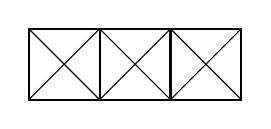
\begin{tikzpicture}[scale=0.9]
\foreach \x in {0,1,2} {\draw[thick] (\x,0) rectangle (\x+1,1); \draw (\x,0)--(\x+1,1); \draw (\x,1)--(\x+1,0);}
\end{tikzpicture}

%% Q36
\textbf{Triangles.} Each square with both diagonals contains 4 small triangles and 4 half-square triangles, i.e.\ $8\times3=24$. Across each pair of adjacent squares, the diagonals meeting at the shared top (or bottom) corner form a larger triangle on the base of two squares: $2$ pairs $\times$ $2$ (top and bottom) $=4$. Total $=\mathbf{28}$.

\textbf{Squares.} There are 3 visible squares. Around each shared vertical edge, the diagonals of the two neighbouring squares form a tilted square (a diamond), which adds 2 more. Total $=\mathbf{5}$.

%% Q37
The official key treats \textbf{census data as primary data}: they are collected directly, first-hand, from every unit of the population by the census organisation. (For other researchers who later use published census tables, the same data become secondary data.)

%% Q38
Blood groups (A, B, AB, O) are \textbf{categories}, not measurements, so they are \textbf{qualitative (nominal)} data.

%% Q39 fig
\begin{tikzpicture}\pie[radius=1.4,text=pin,font=\scriptsize,hide number,color={brand!25,brand!10,brand!35,brand!15,brand!5}]{30/Food 108\textdegree,20/Rent 72\textdegree,20/Clothing 72\textdegree,20/Misc.\ 72\textdegree,10/Savings}\end{tikzpicture}

%% Q39
Savings $=360^\circ-(108+72+72+72)^\circ=36^\circ$.
\[\text{Savings}=\frac{36}{360}\times60{,}000=\mathbf{6{,}000}\]

%% Q40 fig
\begin{tikzpicture}
\begin{axis}[ybar,width=10cm,height=4.4cm,bar width=9pt,ymin=0,ymax=52,
  symbolic x coords={Jan,Feb,Mar,Apr,May,Jun},xtick=data,legend style={font=\tiny,at={(1.02,1)},anchor=north west},
  nodes near coords,every node near coord/.append style={font=\tiny},tick label style={font=\scriptsize},
  ylabel={\scriptsize Registrations ('000)},axis x line*=bottom,axis y line*=left]
\addplot[fill=white,draw=ink] coordinates {(Jan,21) (Feb,15) (Mar,22) (Apr,20) (May,17) (Jun,28)};
\addplot[pattern=north east lines,draw=ink] coordinates {(Jan,27) (Feb,22) (Mar,25) (Apr,35) (May,35) (Jun,45)};
\legend{Cars,Total vehicles}
\end{axis}
\end{tikzpicture}

%% Q40 after
What was the percentage increase in registration of CARS from MAY to JUNE 2004?

%% Q40
Cars: May $=17$ thousand, June $=28$ thousand.
\[\frac{28-17}{17}\times100=\frac{11}{17}\times100\approx\mathbf{64.7\%}\]

%% Q41
The data show male and female numbers (and totals) for each faculty over several years, i.e.\ several related quantities side by side for each category. A \textbf{multiple (grouped) bar diagram} represents this best.
\why{A simple bar diagram shows one variable; a histogram is for continuous frequency distributions; a pie diagram shows the parts of one whole.}

%% Q42
Raw data on height, weight, BMI and age can first be \textbf{classified} (grouped into classes) and then \textbf{tabulated} (arranged in rows and columns) for analysis.

%% Q43
\textbf{Google Chrome} is a web browser.
\why{Windows 7 is an operating system, C++ is a programming language, and Tally is accounting software.}

%% Q44
\textbf{MOOC} is \textbf{Massive Open Online Course}, an online course open to unlimited participants (e.g.\ SWAYAM, Coursera, edX).

%% Q45
Computers store data and compute in the \textbf{binary} number system (0 and 1), matching the two states of electronic circuits.

%% Q46
Crimes committed through computers and the Internet are dealt with by \textbf{cyber law}. In India this is chiefly the Information Technology Act, 2000 (amended in 2008).

%% Q47
\textbf{ATM} is \textbf{Automated Teller Machine}.

%% Q48
\textbf{Encryption} converts data into a coded (cipher) form that only authorised parties with the key can read, e.g.\ SSL/TLS (HTTPS). This secures personal data in transit.

%% Q49
Corrosion (e.g.\ rusting of iron) is an \textbf{electrochemical} process. Anodic and cathodic regions form on the metal surface, with oxidation $\mathrm{Fe}\rightarrow\mathrm{Fe}^{2+}+2e^-$ and reduction of oxygen, and moisture acts as the electrolyte.

%% Q50
The \emph{12 Principles of Green Chemistry} (Anastas \& Warner) include designing safer (benign) chemicals, reducing hazardous substances and \textbf{designing for degradation}: products should break down into harmless substances after use. ``Design for \emph{non}-degradation'' is therefore not correct.

%% Q51
\textbf{Har Gobind Khorana} shared the 1968 Nobel Prize in Physiology or Medicine (with Nirenberg and Holley) for the \textbf{interpretation (cracking) of the genetic code} and its role in protein synthesis.

%% Q52
\textbf{COD (Chemical Oxygen Demand)} measures the oxygen needed to chemically oxidise organic pollutants in water. It is an indicator of organic pollution (together with BOD).

%% Q53
Chewing-gum and bubble-gum bases use synthetic elastomers, mainly \textbf{styrene--butadiene rubber (SBR)} and polyisobutylene, which give them stretch and elasticity.

%% Q54
\textbf{World Environment Day} is celebrated on \textbf{5 June} every year (UNEP; first observed in 1974, commemorating the 1972 Stockholm Conference).

%% Q55
The main objective of \textbf{NAAC} is the \textbf{assessment and accreditation} of higher-education institutions.

%% Q56
\textbf{Gujarat Vidyapith}, founded by Mahatma Gandhi in 1920, is a \textbf{deemed university} (since 1963).

%% Q57
\textbf{INSPIRE} (Innovation in Science Pursuit for Inspired Research, 2008) is DST's flagship programme to attract young talent to science through scholarships, fellowships and awards (e.g.\ INSPIRE-MANAK).

%% Q58
\textbf{Banaras Hindu University} (founded 1916 by Madan Mohan Malaviya) is a central university.
\why{Gujarat University, Mohanlal Sukhadia University (Udaipur) and the University of Mumbai are state universities.}

%% Q59
\textbf{SNDT Women's University}, Mumbai (founded 1916 by Dhondo Keshav Karve) is India's first exclusively women's university.

%% Q60 note
The official key gives (A). Students should note that the best-known \emph{Vikram Sarabhai Research Award} (Physical Research Laboratory) and the \emph{Vikram Sarabhai Memorial Award} (COSPAR) relate to space science. Answer as per the key in the exam context.

%% Q60
Awards named after Dr.~Vikram Sarabhai, the father of India's space programme, are given in several fields of science. The official GSET key identifies the field as \textbf{biological research}.
